\documentclass[12pt]{article}
\usepackage{graphicx,import}
\usepackage[svgnames]{xcolor} 
\usepackage{fancyhdr}
\usepackage{subfig}
\usepackage{hyperref}
\usepackage{enumitem}
\usepackage{cite}
\usepackage[many]{tcolorbox}
\usepackage{listings }
\usepackage[a4paper, total={6in, 8in} , bottom = 25mm , top = 25mm, headheight = 1.25cm , includehead,includefoot,heightrounded ]{geometry}
\usepackage{afterpage}
\usepackage{amssymb}
\usepackage{pdflscape}
\usepackage{gensymb}
\usepackage{textcomp}
\usepackage{xecolor}
\usepackage{rotating}
\usepackage{pdfpages}
\usepackage[Kashida]{xepersian}
\usepackage[T1]{fontenc}
\usepackage{tikz}
\usepackage[utf8]{inputenc}
\usepackage{PTSerif} 
\usepackage{seqsplit}

\usepackage[edges]{forest}

\usepackage{listings}
\usepackage{xcolor}

\hypersetup{
	colorlinks   = true, %Colours links instead of ugly boxes
	urlcolor     = blue, %Colour for external hyperlinks
	linkcolor    = blue, %Colour of internal links
	citecolor   = red %Colour of citations
}
 
\definecolor{codegreen}{rgb}{0,0.6,0}
\definecolor{codegray}{rgb}{0.5,0.5,0.5}
\definecolor{codepurple}{rgb}{0.58,0,0.82}
\definecolor{backcolour}{rgb}{0.95,0.95,0.92}
 
\NewDocumentCommand{\codeword}{v}{
\texttt{\textcolor{blue}{#1}}
}
\lstset{language=java,keywordstyle={\bfseries \color{blue}}}

\lstdefinestyle{mystyle}{
    backgroundcolor=\color{backcolour},   
    commentstyle=\color{codegreen},
    keywordstyle=\color{magenta},
    numberstyle=\tiny\color{codegray},
    stringstyle=\color{codepurple},
    basicstyle=\ttfamily\normalsize,
    breakatwhitespace=false,         
    breaklines=true,                 
    captionpos=b,                    
    keepspaces=true,                 
    numbers=left,                    
    numbersep=5pt,                  
    showspaces=false,                
    showstringspaces=false,
    showtabs=false,                  
    tabsize=2
}

\lstset{style=mystyle}

\settextfont[Scale=1.2 ,BoldFont={Bahij Nazanin-Bold.ttf} , ItalicFont = {IRNazaninIranic.ttf}]{Bahij Nazanin-Regular.ttf}
\setlatintextfont[Scale = 1.0]{Garamond}
\DefaultMathsDigits 
\DeclareMathSizes{11}{19}{13}{9} 
%\DeclareMathSizes{12}{14.4}{8}{9}





\newenvironment{changemargin}[2]{%
\begin{list}{}{%
\setlength{\topsep}{0pt}%
\setlength{\leftmargin}{#1}%
\setlength{\rightmargin}{#2}%
\setlength{\listparindent}{\parindent}%
\setlength{\itemindent}{\parindent}%
\setlength{\parsep}{\parskip}%
}%
\item[]}{\end{list}}


\definecolor{foldercolor}{RGB}{124,166,198}

\tikzset{pics/folder/.style={code={%
    \node[inner sep=0pt, minimum size=#1](-foldericon){};
    \node[folder style, inner sep=0pt, minimum width=0.3*#1, minimum height=0.6*#1, above right, xshift=0.05*#1] at (-foldericon.west){};
    \node[folder style, inner sep=0pt, minimum size=#1] at (-foldericon.center){};}
    },
    pics/folder/.default={20pt},
    folder style/.style={draw=foldercolor!80!black,top color=foldercolor!40,bottom color=foldercolor}
}

\forestset{is file/.style={edge path'/.expanded={%
        ([xshift=\forestregister{folder indent}]!u.parent anchor) |- (.child anchor)},
        inner sep=1pt},
    this folder size/.style={edge path'/.expanded={%
        ([xshift=\forestregister{folder indent}]!u.parent anchor) |- (.child anchor) pic[solid]{folder=#1}}, inner xsep=0.6*#1},
    folder tree indent/.style={before computing xy={l=#1}},
    folder icons/.style={folder, this folder size=#1, folder tree indent=3*#1},
    folder icons/.default={12pt},
}

\begin{document}


%%% title pages
\begin{titlepage}
\begin{center}
        
\vspace*{0.7cm}


\includegraphics[width=0.4\textwidth]{sharif1.png}\\
\vspace{0.5cm}
\textbf{ \Huge{\emph ‌اندازه‌گیری و کنترل کامپیوتری} }\\
\vspace{0.5cm}
\textbf{ \Large{ تمرین دوم} }
\vspace{0.2cm}
       
 
      \large \textbf{دانشکده مهندسی کامپیوتر}\\\vspace{0.2cm}
    \large   دانشگاه صنعتی شریف\\\vspace{0.2cm}
       \large   ﻧﯿﻢ سال دوم 00-99 \\\vspace{0.2cm}
      \noindent\rule[1ex]{\linewidth}{1pt}
استاد:\\
    \textbf{{جناب آقای دکتر همت‌یار}}


    \vspace{0.15cm}
نام و نام خانوادگی:\\

       
    \textbf{{امیرمهدی نامجو - 97107212}}
\end{center}
\end{titlepage}
%%% title pages


%%% header of pages
\newpage
\pagestyle{fancy}
\fancyhf{}
\fancyfoot{}
\cfoot{\thepage}
\chead{تمرین دوم}
\rhead{
\includegraphics[width=0.1\textwidth]{sharif.png}}
\lhead{امیرمهدی نامجو}
%%% header of pages

\KashidaOff


\section*{سوال 4}

برای مثال $2$ کتاب طبق راه‌حل نوشته شده در خود کتاب فرمول به این صورت است:

$$V = \frac{5R_2}{10000 + R_2}$$

با رسم آن در بازه $500\Omega$ تا $20k\Omega$ داریم:

\begin{center}
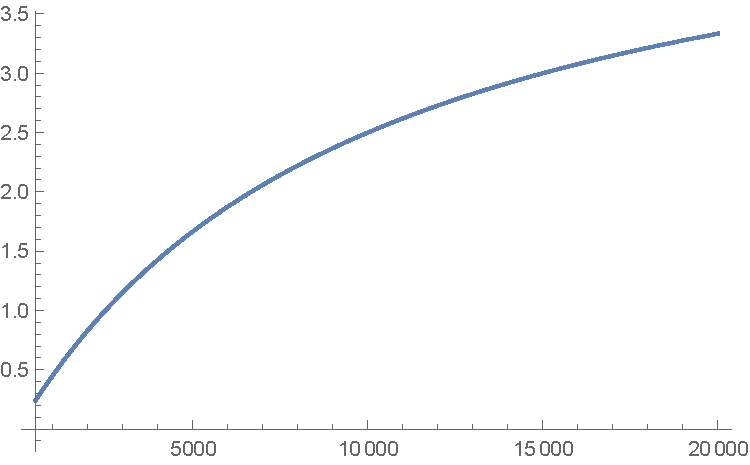
\includegraphics[width = 0.5\textwidth]{images/1.pdf}
\end{center}
مبدا مختصات روی
$(500 , 0)$
است.

برای قسمت بعدی، با توجه به اعداد سوال $3$ فرمول بدین صورت است:

$$V = \frac{10\times 500}{500 + R_1}$$

با رسم آن در همان بازه قبلی به شکل زیر می‌رسیم:

\begin{center}
	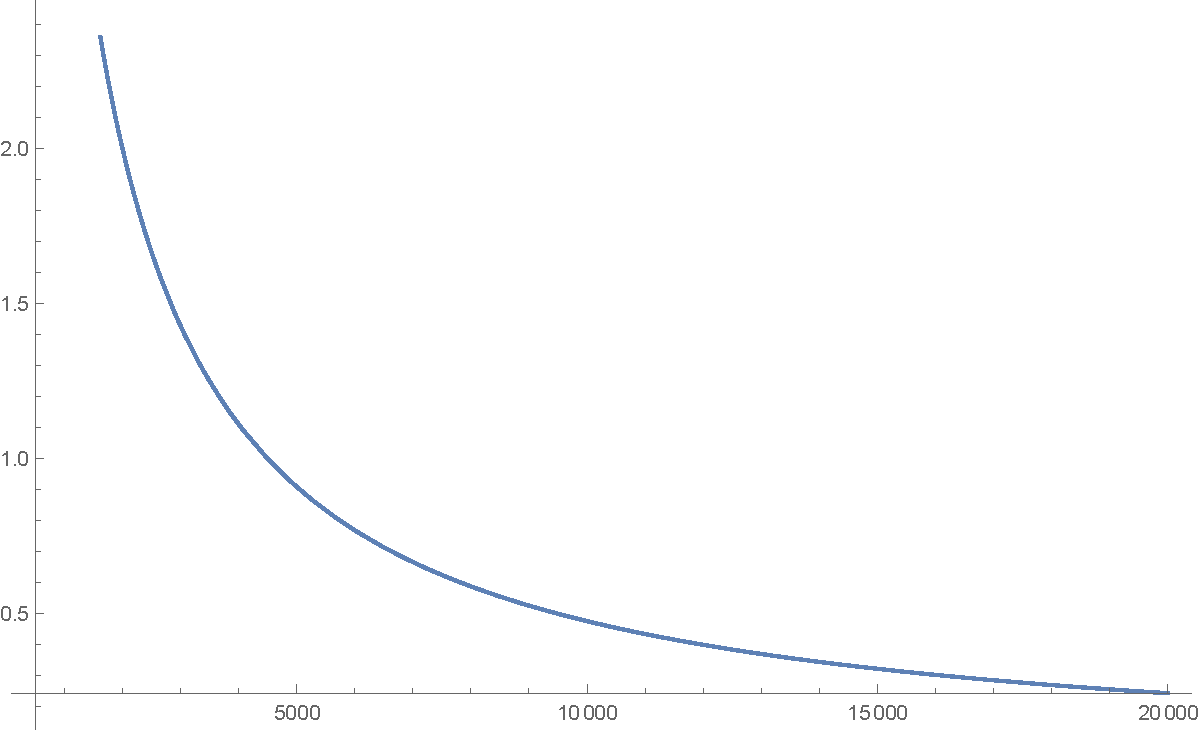
\includegraphics[width = 0.5\textwidth]{images/2.pdf}
\end{center}

مبدا مختصات در این شکل $(0,0)$ است.

در هر دو حالت غیرخطی است. در اولی با افزایش مقاومت، افزایش ولتاژ داریم و در دومی با افزایش مقاومت، کاهش ولتاژ داریم.

شکل‌ها با نرم افزار Mathematica رسم شده‌اند.

\newpage

\section*{سوال 8}

صورت سوال کمی گنگ است. به نظر می‌رسد که سوال $R_3$ را خواسته است اما خودش $R_3$ را داده است! به هر حال فرض می‌کنیم $R_4 = 50\Omega$ بوده و $R_3$ مجهول بخش الف باشد.

\begin{enumerate}[label = \harfi*)]
	\item 
	برای این قسمت داریم:
	$$R_1 R_3 = R_2 R_4 \rightarrow R_3 = \frac{50 \times 100}{100} = 50 \Omega$$
	
	\item
	
	برای این قسمت طبق فرمول $6$ صفحه $63$، 
	$\Delta V$
	را برای نوسان $0.1 \Omega$ ای در $R_4$ محاسبه می‌کنیم.
	
	
	$$
	\Delta V=\frac{V R_{3}}{R_{1}+R_{3}}-\frac{V R_{4}}{R_{2}+R_{4}}
	$$
	
	اگر براساس افزایش مقاومت حساب کنیم:
	
	$$\Delta V = \frac{10 \times 50}{(50 + 100)} - \frac{10 \times 50.1}{(50.1 + 100)} = -44.4 mV$$
	
	در صورتی که با کاهش مقاومت حساب کنیم:
	
		$$\Delta V = \frac{10 \times 50}{(50 + 100)} - \frac{10 \times 49.9}{(49.9 + 100)} = +44.47 mV \approx 44.5 mV$$
		
		
\end{enumerate}

\newpage

\section*{سوال 12}

مطابق فرمول صفحه 70 عمل می‌کنیم:

$$
V_{x}+\frac{R_{3} V}{R_{1}+R_{3}}-\frac{V R_{4}}{R_{2}+R_{4}}=0
$$

$$V_{x} = \frac{10 \times 9.73}{10+9.73} - \frac{10 \times 10}{10+10} = -0.0684 V = -68.4 mV$$


و معنای علامت منفی‌ هم این است که پتانسیل $c$ در شکل 9 کتاب مطابق این مسئله کمتر از پتانسیل $a$ شده است.

\newpage

\section*{سوال 16}

$$
\left|\frac{V_{\text {out }}}{V_{\text {in }}}\right|=\frac{1}{\left[1+\left(f / f_{c}\right)^{2}\right]^{1 / 2}}
$$

$$\left|\frac{V_{\text {out }}}{V_{\text {in }}}\right| = \frac{1}{\sqrt{1 + (1/3.5)^2}} = 0.96152$$

در نتیجه این نشان‌دهنده تضعیف به اندازه
$1 - 0.96152 = 0.03848$
است.


\newpage

\section*{سوال 20}

شکل اولیه مسئله به این صورت می‌شود.

\begin{center}
	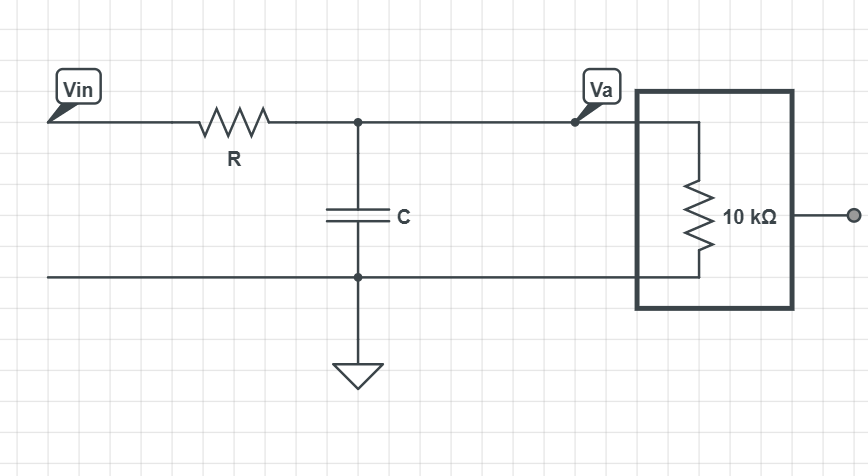
\includegraphics[width = 0.5\textwidth]{images/3.png}
\end{center}

نکته ای که وجود دارد این است که قطعه سمت راست روی مدار لود می‌اندازد و باید این موضوع هم در نظر گرفته شود. در نتیجه شکل دوم را براساس مقاومت معادل به این شکل می‌کشیم:

\begin{center}
	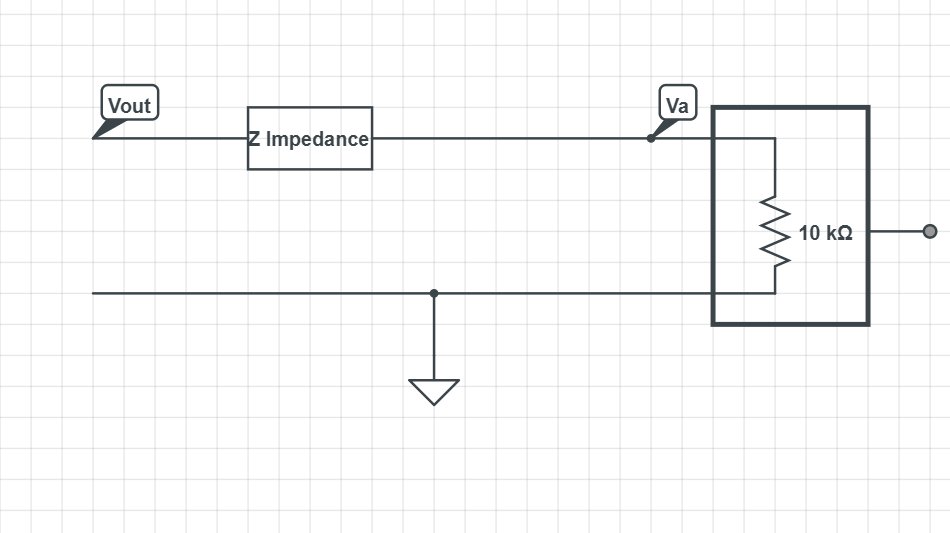
\includegraphics[width = 0.5\textwidth]{images/4.png}
\end{center}

سوال از ما می‌خواهد که برای فرکانس ۲۰۰ هرتز
$|\frac{va}{vin}| >0.99$
باشد. از طرفی در این جا دو تبدیل داریم. یکی تبدیل $vin$ به $vout$ و دومی تبدیل $vout$ به $va$ است. به نوعی حاصل ضرب
$|\frac{va}{vout}| |\frac{vout}{vin}| > 0.99$
باید بشود. از آن جایی که جذر $0.99$ تقریبا برابر $0.995$ است فرض می‌کنیم هر کدام از این تبدیل‌ها با ضریب $0.995$ انجام بشوند. داریم:

$$
\frac{V_{\text {out }}}{V_{\text {in }}}=\frac{1}{\sqrt{1+\left(f / f_{c}\right)^{2}}}
$$

$$
\left|\frac{V_{a}}{V_{\text {out }}}\right|=\frac{10 k+0 j}{\left|10 k+Z\right|}
$$

که رابطه دوم به این دلیل مختلط نوشته شده که $Z$ مختلط خواهد شد و رابطه براسا تقسیم ولتاژ سری نوشته شده است. حال با فرض
$\frac{V_{\text {out }}}{V_{\text {in }}} = 0.995$
و برای $f=200hz$ مقدار $f_c$ را پیدا می‌کنیم:

$$
0.995=\frac{1}{\sqrt{1+\left(200 / f_{c}\right)^{2}}} \Rightarrow f_c = 1992.5 hz
$$

برای بدست آوردن امپدانس معادل اگر فقط مدار سمت چپ را در نظر بگیریم و منبع را هم صفر کنیم تا مدار معادل تونن بگیریم، می بینیم $R$ و $C$ موازی اند. در نتیجه:
$$Z = \frac{1}{R} + j\Omega C = \frac{R}{1 + Rj\Omega C}$$

از طرفی
$RC = \frac{1}{2 \pi f_c} , \Omega = 2 \pi f$

در نتیجه با عدد گذاری و ساده سازی عبارت مختلط داریم:

$$
Z_{f}=0.99 R(1-0.1004 j)
$$

همچنین

$$
\frac{V_{a}}{V_{\text {out }}}=0.995=\frac{10000}{|10000+0.99 R(1-0.1004 j)|}
$$


از حل کامپیوتری آن داریم:
$R = 50.76 \Omega$.
البته یک جواب حدود $R=-20000 \Omega$ هم تولید می‌شود که غیر منطقی است.

$$C = \frac{1}{ 2 \pi R f_c} = 1.57 \mu F$$

برای بدست آوردن تضعیف برای سیگنال‌های داده شده داریم:

$$|\frac{v_a}{v_{in}}| = |\frac{v_{out}}{v_{in}}| |\frac{v_a}{v_{out}}| = \frac{1}{\sqrt{1+\left(f / f_{c}\right)^{2}}} \times 0.995 $$

$$f = 4000 \Rightarrow |\frac{v_a}{v_{in}}| = 0.4436$$

$$f = 5000 \Rightarrow |\frac{v_a}{v_{in}}| = 0.3683$$

\newpage

\section*{سوال 24}

مطابق شکل صفحه $96$ کتاب و فرمول بهره در Diif.Amp داریم:
$\frac{R_2}{R_1} = 22 $

از آن جایی که بهتر است مقاومت ها را خیلی کوچک نگیریم به این صورت در نظر می‌گیریم:
$R_1 = 1 k\Omega , R_2 = 22 k \Omega$

شکل آن بدین صورت می‌شود:


\begin{center}
	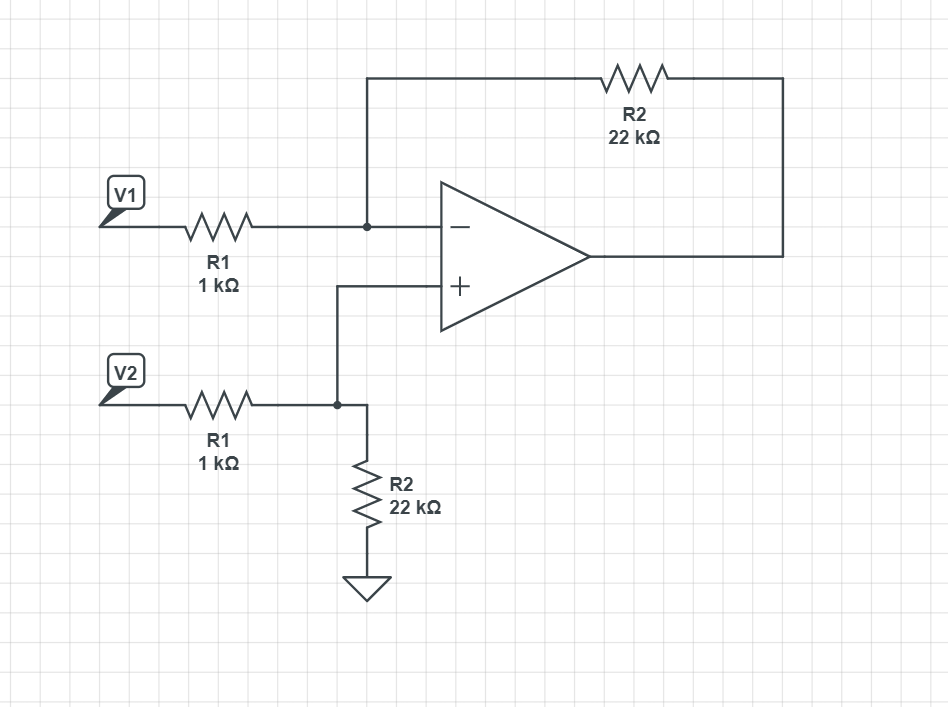
\includegraphics[width = 0.5\textwidth]{images/5.png}
\end{center}

\newpage

\section*{سوال 28}

با توجه به نامگذاری شکل زیر حل می‌کنیم:

\begin{center}
	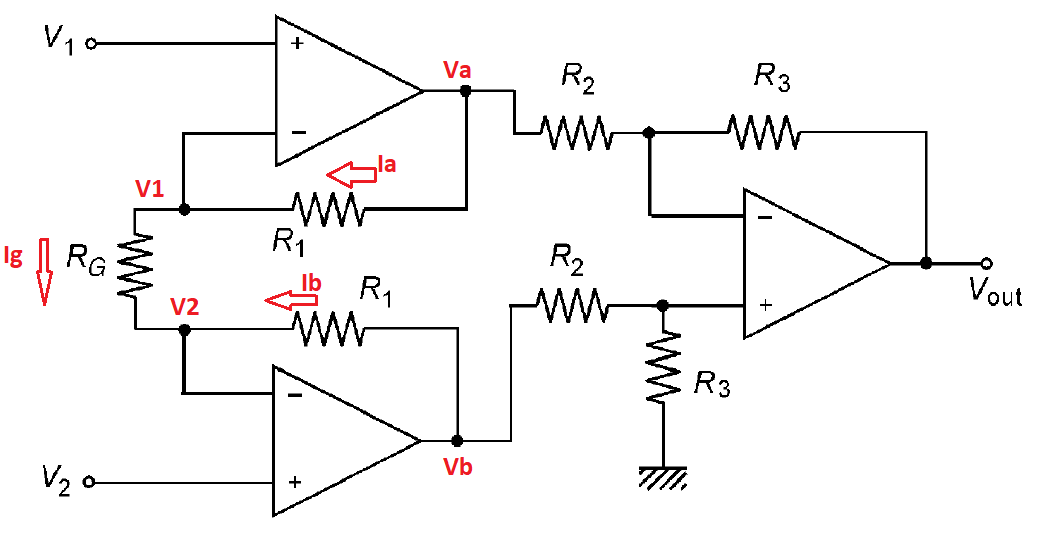
\includegraphics[width = 0.5\textwidth]{images/6.png}
\end{center}

$$I_g = \frac{V_1 - V_2}{R_G} ; \text{قانون اهم}$$
$$I_g = I_a , I_g = -I_b ; \text{KCL}$$
$$V_a = V_1 + \frac{R_1}{R_G} (V_1 - V_2) , V_b = V_2 - \frac{R_1}{R_G}(V_1 - V_2) ; \text{KVL}$$

$$V_{out} = \frac{R_3}{R_2} (V_b - V_a) = \frac{R_3}{R_2}; \text{فرمول \lr{Differntial Amplifier}}$$

$$V_{out} = ((V_2 - V_1) + \frac{2R_1}{R_G} (V_2 - V_1)) \frac{R_3}{R_2} $$

$$
V_{\text {out }}=\left(1+\frac{2 R_{1}}{R_{G}}\right)\left(\frac{R_{3}}{R_{2}}\right)\left(V_{2}-V_{1}\right)
$$
\newpage

\section*{سوال 32}


طبق فرمول‌های تبدیل کننده ولتاژ به جریان داریم:

$$\frac{R_2}{R_1 R_3} = 2.1 \times 10^{-3}$$
$$
R_{1}\left(R_{3}+R_{5}\right)=R_{2} R_{4}
$$

پنج مجهول و دو معادله داریم. مقادیر $R_3$ و $R_1$ را ابتدا 
$1 k\Omega$
می گذاریم که به راحتی
$R_2 = 2.1 k \Omega$
بدست بیاید.

حال فرض کنید 
$R_5 = 1 k \Omega$
بگیریم. در آن صورت داریم:

$$R_4 = \frac{1000 \times (1000 + 1000)}{2100}= 952.38 \Omega$$


برای قسمت بعدی سوال داریم:

$$
R_{M L}=\frac{\left(R_{4}+R_{5}\right)\left(V_{s a t} / l_{M}-R_{3}\right)}{\left(R_{3}+R_{4}+R_{5}\right)}
$$

در نتیجه:

$$R_{ML} = \frac{(952.38+1000)(\frac{12}{0.005} - 1000)}{1000+952.38+1000} = 925.806 \Omega$$

\newpage

\section*{سوال 36}

$$V_{out} = m R + V_0$$

$$0 = m(1 k \Omega) + V_0)$$
$$5 = m(5 k \Omega) + V_0)$$

از معادلات بالا داریم:
$m = 1.25 V/k\Omega , V_0 = -1.25$
یعنی
$$V_{out} = 1.25 R - 1.25$$

این مدار را می‌توان از ترکیب یک مدار معکوس کننده و یک مدار جمع کننده ساخت. در اصل در مدار معکوس کننده داریم
$V_out = -\frac{R_2}{R_1} V_{in}$
و در این جا $R_2 =R$ گذاشته و $V_in$ را روی $1.25 V$ تنظیم می‌کنیم. این تنظیم را از طریق مدار ساده تقسیم کننده ولتاژ روی مقاومت انجام می‌دهیم که از $5$ ولت تغذیه، خروجی $1.25$ ولت بگیرد.. از آن جایی که در مدار جمع کننده در نهایت فرمول $V_{\text {out }}=-\left[\frac{R_{2}}{R_{1}} V_{1}+\frac{R_{2}}{R_{3}} V_{2}\right]$ را داریم، یک بار دیگر منفی ضرب خواهد شد و عبارت ضریب $R$ مثبت می‌شود. برای جمع کننده هم ضرایب نسبت‌های $R$ ها را یکسان می‌گذاریم که صرفا جمع ساده بزند.

در نهایت مدار زیر می‌تواند یکی از پیاده‌سازی‌های ممکن برای این سوال باشد. (امکان زوم‌کردن روی شکل وجود دارد)


\begin{center}
	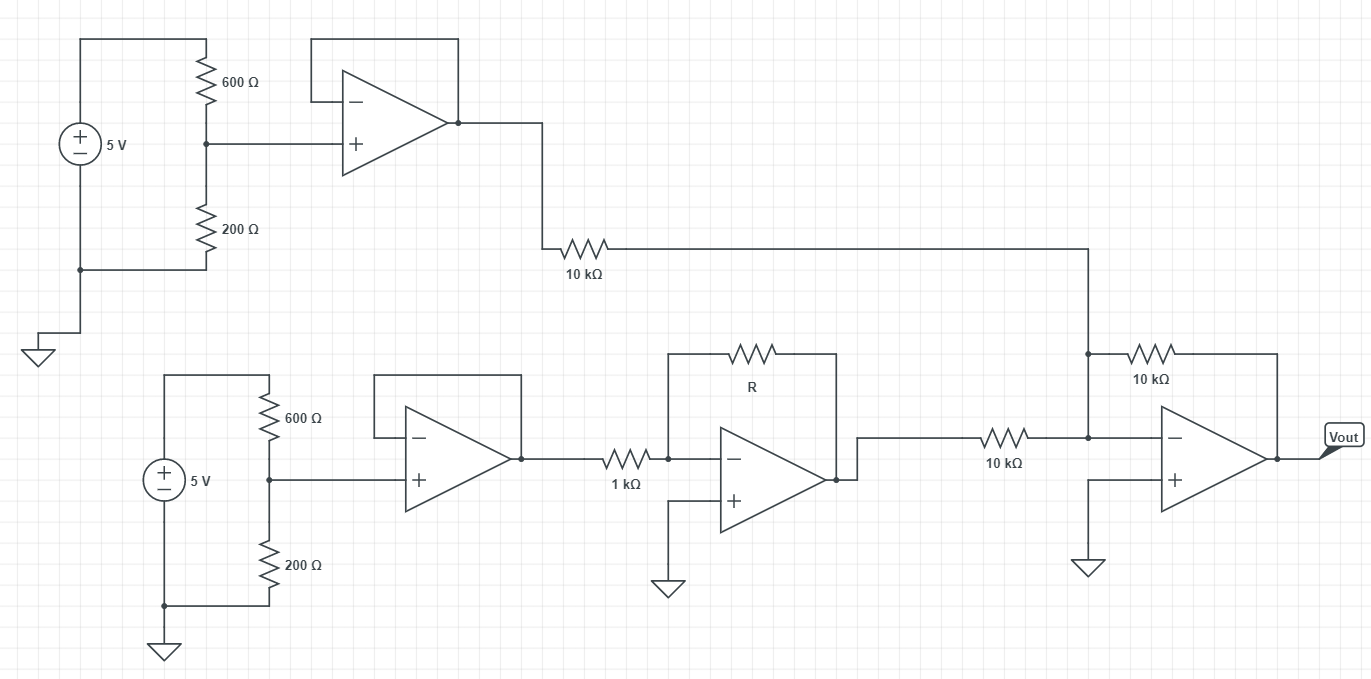
\includegraphics[width = 0.9\textwidth]{images/7.png}
\end{center}

توجه کنید که دنبال کننده ولتاژ هم در این شکل قرار داده شده است تا جلوی لود انداختن بقیه مدار روی منبع تغذیه و تقسیم کننده ولتاژ گرفته شود.

مقاومت $1k\Omega$ برای مدار معکوس کننده پایین برای این قرار داده شده است که ضریب تقسیم $V/k\Omega$ که در واحد‌های سوال آمده ایجاد شود. ضرایب $10k\Omega$ ای مدار جمع‌کننده دلخواه هستند و صرفا عدد نسبتا بزرگ و رند گذاشته شده است که از عملکرد صحیح اپ امپ مطمئن باشیم.


\section*{سوال 40}

$$Q1 = 20 gal/min \Rightarrow V_1 = \sqrt{Q1} = 4.472 V$$
$$Q2 = 30 gal/min \Rightarrow V_2 = \sqrt{Q2} = 5.477 V$$

همچنین فرکانس تغییر ولتاژ (و شار) مد نظر ما به صورت $1/30 = 0.033 Hz$ است. از طرفی نویز ما $60Hz$ است در نتیجه می‌توانیم از فیلتر Low-Pass استفاده کنیم. فرض می‌کنیم این فیلتر $99$ درصد نویز را بگیرد. بر این اساس $f_c$ را پیدا می‌کنیم:

$$0.01 = \frac{1}{\sqrt{(1 + (60 / f_c)^2)}} \Rightarrow f_c = 0.6 Hz \Rightarrow RC = \frac{1}{0.6 \times Pi \times 2} = 0.265$$

حالا باید تنظیم کردن بین ولتاژ $-2.5$ تا $2.5$ ولت را انجام بدهیم. ابتدا باید ببینم خروجی مدار فیلتر کننده برای ولتاژهایی که در ابتدا بدست آوردیم و فرکانس $0.033$ هرتز چند خواهد بود. این دو را $V'_1$ و $V'_2$ می‌نامیم.

$$V'_1 = \frac{4.472}{\sqrt{(1 + (0.033/0.6)^2)}} = 4.465 V$$

$$V'_2 = \frac{5.477}{\sqrt{(1 + (0.033/0.6)^2)}} = 5.468 V$$

حال داریم:

$$V_{out} = m V_{in} + V_0$$

$$-2.5 = m \times (4.465) + V_0$$
$$+2.5 = m \times (5.468) + V_0$$

با حل دستگاه داریم:

$$V_{out} = 4.985 V_{in} -24.758  = 4.985(V_{in} - 4.966)$$

برای طراحی چنین سیستمی از \lr{Instrumentation Amplifier} استفاده می‌کنیم. همچنین با توجه به این که مقدار $2 k \Omega$ که خروجی سنسور است کوچک است، باید یک دنبال کننده ولتاژ هم در آن جا قرار بدهیم که ادامه مدار روی آن لود نیندازد.

برای طراحی مدار Low-Pass از $C=1 \mu F$ و $R = 265 k \Omega$ استفاده می‌کنیم.

نتیجه نهایی به این صورت خواهد بود:



\begin{center}
	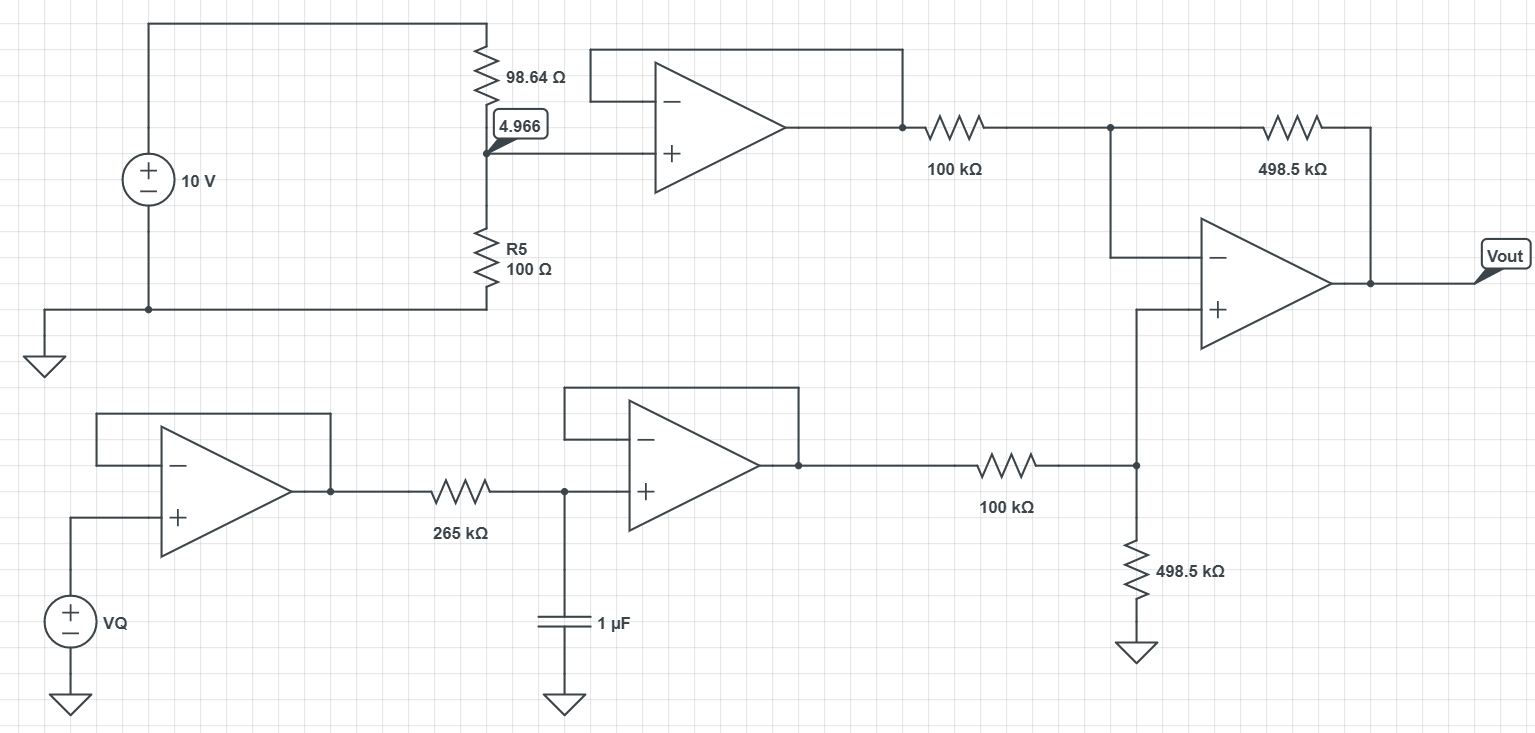
\includegraphics[width = 0.9\textwidth]{images/8.png}
\end{center}

فرض کرده‌ایم که یک منبع تغذیه $10V$ در اختیار داشته باشیم. منظور از $VQ$ در شکل هم خروجی سنسور است.

جواب بخش نمودار:
فرمول نهایی سوال به این صورت می‌شود:

$$V_{out} =  4.985( \frac{\sqrt{Q}}{\sqrt{1 + (0.033/0.6)^2}} - 4.966)$$

نمودار آن در زیر آمده است. مبدا مختصات در شکل
 $(20,0)$
  است.


\begin{center}
	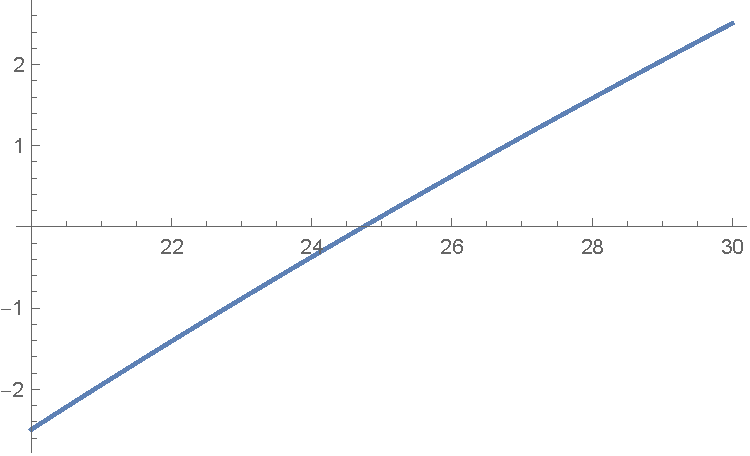
\includegraphics[width = 0.5\textwidth]{images/3.pdf}
\end{center}

برای قسمت آخر سوال که درصد Full-Scale نویز را خواسته است داریم:

$$\frac{0.8}{\sqrt{1 + (60/0.6)^2}} = 0.008 V$$

از آن جایی که بازه ولتاژی ما از $-2.5$ تا $2.5$ و به عبارتی $5$ ولت است، درصد Full-Scale برابر خواهد بود با:

$$\frac{0.008}{5} \times 100=0.16\%$$

 
\end{document}



